\section{Javascripts.}

\subsection{Qué es.}

Mozilla, los herederos directos de Netscape, definen Javascripts como:\footnote{MDN (Mozilla Developer Network)} \footnote{https://developer.mozilla.org/en-US/docs/Web/JavaScript/Guide/JavaScript\_Overview}

\begin{quotation}
Javascripts is a cross-platform, object-oriented scripting language. JavaScript is a small, lightweight language; it is not useful as a standalone language, but is designed for easy embedding in other products and applications, such as web browsers. Inside a host environment, JavaScript can be connected to the objects of its environment to provide programmatic control over them.
\end{quotation}

Definición que desde mi punto de vista se queda corta. Ya que Javascripts es un lenguaje de scripting (que debe ser interpretado), imperativo, estructurado, orientado a objeto sin clases, débilmente tipado, dinámico, funcional y basado en prototipos.

De C ha heredado que sea un lenguaje imperativo y estructurado con distinción entre sentencias y expresiones. A diferencia de C y Java el ámbito de las variables no son a nivel de bloque sino de función, es decir, que una variable definida dentro de una sentencia puede ser utilizada fuera de dicha sentencia, ya que el ámbito no lo define la sentencia sino la función que la contiene.

\begin{lstlisting}[language=JavaScript, numbers=left]
var f = function (valor) {
	if ( valor ) {
		var resultado = 'Si';
	} 
	return resultado;
};
\end{lstlisting}

Sin lugar a dudas se trata de un lenguaje orientado a objeto. Los arrays, números, funciones, cadenas, casi en su totalidad el lenguaje son objetos\footnote{Salvo los valores destacados null y undefined, el resto de valores Javascripts son objetos}. Los objetos son array asociativos al cual podemos acceder a través de la notación objeto.campo o como si de un array se tratará. 

\begin{lstlisting}[language=JavaScript, numbers=left]
var f = function () {
	var objeto = { 
		campo0 : 0,
		campo1 : 'una cadena' 
	};
	
	var valorCampo0 = objeto.campo0;
	valorCampo0 = objecto['campo0'];
};
\end{lstlisting}

Es débilmente tipado, el tipo no va asociado a la variable si al valor que contiene. Por lo que podemos crear variables y asignarle un valor numérico y posteriormente una cadena. 

\begin{lstlisting}[language=JavaScript, numbers=left]
var f = function () {
	var numero = 1;
	numero++;
	numero = '1';
};
\end{lstlisting}

Se trata de un lenguaje funcional en el que una función es un objeto de primera clase. Esto significa que Javascripts soporta el paso de funciones como argumentos a otras funciones, funciones que devuelve funciones, variables que almacenan funciones, creación de funciones anónimas, etc ...

\begin{lstlisting}[language=JavaScript, numbers=left]
function map(f, xs) {
	var result = new Array();
	for (var i = 0; i < xs.length; i++)
		result.push(f.apply(null, [xs[i]]));
	return result;
}
\end{lstlisting}

Javascripts no utiliza los mecanismos de clases para implementar la herencia, para ello hace uso de los prototipos. 

\begin{lstlisting}[language=JavaScript, numbers=left]
var Persona = function (){
	this.nombre = 'Sin nombre';
};

Persona.prototype.setNombre = function () {
	this.nombre;
};

var pepe = new Persona(); // pepe es una instancia de Persona 
pepe.setNombre('Pepe');   // y contiene una copia del prototipo de Persona.
\end{lstlisting}


\subsection{Un poco de historia.}

Cuando en 1996, el navegador Netscape introdujo su primer interprete de
Javascripts\footnote{Javascripts fue un nombre por conveniencia legal. Originalmente se llamaba
  LiveScript} nadie podía intuir la importancia que adquiriría años después. 

Internet aun estaba en pañales, navegar era lento\footnote{La velocidad máxima de los modems de
  usuario era 28.8Kbps} y los ordenadores personales poco potentes. En el mejor de los casos, el
usuario tenía que esperar durante largo tiempo para poder interactuar con la web solicitada.  Las
páginas comenzaban a ser más complejas, y la navegación más lenta, de ello surgió la necesidad de
un lenguaje de programación que se ejecutará en el navegador del cliente. De esta forma, si el
usuario introducía un valor incorrecto, en un formulario, no tendría que esperar a la respuesta del
servidor, el mismo cliente podría dar una respuesta más rápida, indicando los errores existentes.

Netscape Navigator 3.0 incorporó la primera versión del lenguaje, como ya se había comentado, y al
mismo tiempo, o al poco, Microsofot lanzo JScript en su Internet Explorer 3. JScript no era más que 
una copia de Javascripts al que le cambiaron el nombre para evitar problemas legales. De esta
forma comienzan las divergencias entre las distintas versiones de Javascripts, en esencia todas
parten del mismo lenguaje y estándar, pero cada una aportaba sus mejoras provocando diferencias
entre ellas. 

La guerra entre las distintas versiones estaba servida. Todos deseaban que su versión fuera la
aceptada por la comunidad y se popularizará. Bien intentando estandarizar su versión, o buscando
que se evitará la guerra de tecnologías, Netscape decidió dar el paso, y en 1997 puso a disposición
de ECMA\footnote{European Computer Manufacturers Association. Web oficial
  http://www.ecma-international.org/} la especificación de Javascripts1.1. ECMA creo el comité TC39
del cual surgió el primer estándar que se denominó ECMA-262\footnote{Se puede encontrar la versión 5.1 en
  http://www.ecma-international.org/publications/files/ECMA-ST/ECMA-262.pdf}, o más popularmente, 
ECMAScript. 

Durante mucho tiempo el estándar ECMAScript no fue el aceptado por todos los navegadores, ni que
decir tiene que el más reacio al cambio fue el Internet Explorer de Microsoft. Es ahora, donde
Microsoft a dado su brazo a torcer y poco a poco tiende al estándar ECMAScript facilitando al los
desarrolladores su tarea.

\subsection{Prototipos}

Como se ha comentado con anterioridad Javascripts no utiliza el mecanismos de clases\footnote{Paradigma sin clases} para implementar la herencia, para ello hace uso de los prototipos. Los prototipos son un paradigma de programación orientada a objetos en la cual una instanciación de objetos, se lleva a cabo mediante la clonación de otros objetos. 

Los objetos en cualquier lenguaje son un conjunto de propiedades y métodos. Pues bien, Javascripts carece de métodos en su lugar existen propiedades que apuntan a funciones que hacen las veces de métodos. Además, cada objeto tiene un enlace interno a otro objeto llamado prototipo\footnote{prototype}. El prototipo de un objeto puede ser, o bien otro objeto, o bien el valor null. Es lo que se llama cadena de prototipos o cadena prototípica (ver figura\ref{fig:cadena-prototipos}). 

\begin{figure}[tbph]
\centering
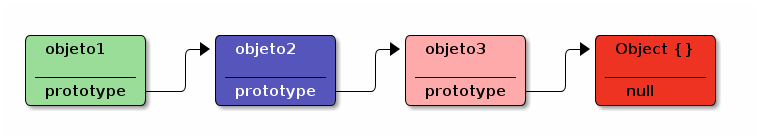
\includegraphics[width=0.7\linewidth]{imagenes/prototipo1}
\caption{Cadena prototípica de objetos}
\label{fig:cadena-prototipos}
\end{figure}

Cómo se puede observar toda cadena de prototipo acaba con el prototipo de Object, cuyo prototipo es null. Veamos algunos ejemplo de cadenas prototípicas. 

\begin{lstlisting}[language=JavaScript, numbers=left]
> var objeto = { a : 1 }; \\ cadena prototípica de objeto --> Object.prototype --> null
> Object.getPrototypeOf(o); 
  Object {}
> Object.getPrototypeOf(Object.getPrototypeOf(o));
  null

\\ cadena prototípica de una array --> Array.prototype --> Object.prototype --> null
> var array = [1,2];
> Object.getPrototypeOf(array);
  []
> Object.getPrototypeOf(Object.getPrototypeOf(array));
  Object {}
> Object.getPrototypeOf(Object.getPrototypeOf(Object.getPrototypeOf(array)));
  null
\end{lstlisting}


\subsubsection{Herencia de propiedades y métodos}

Un objeto Javascripts es un conjunto de propiedades\footnote{Los métodos son propiedades que referencia a una función} que en el momento de la herencia se copian en el nuevo objeto o objeto hijo. Así pues, en el siguiente ejemplo podemos observar como se heredan las propiedades y los "métodos". 

\begin{lstlisting}[language=JavaScript, numbers=left]
> var a = { 
	contador: 0, 
	contar : function () { 
		console.log('Contador ' + this.contador++); 
	} 
};
> a.contar();
  Contador 0
> a.contar();
  Contador 1

> var b = Object.create(a); // Crea un objeto "b" que hereda de "a"
> b.contador; // es una copia exacta de "a"
  2
> b.contar();
  Contador 2
> a.contar();  // una copia no el mismo
  Contador 2

// la cadena de prototipos de los objetos:
// b.prototype --> a.prototype --> Object.prototype --> null
\end{lstlisting}

También hay que tener especial cuidado con la palabra reservada this que siempre apunta al objeto que está heredando y no al prototipo. 

\subsubsection{Constructor, propiedad prototype y herencia}
Todos los objetos poseen un único constructor. Un constructor es sólo una función que ha sido llamada con la palabra reservada new.

Todo constructor tiene una propiedad prototype con la cual podemos definir el prototipo de todos los objetos creados con dicho constructor.

\begin{lstlisting}[language=JavaScript, numbers=left]
> var Persona = function (nombre) { 
	this.nombre = nombre;
};

> Persona.prototype = {
	saluda : function () {
		console.log('Hola soy ' + this.nombre);
	}
};

> var pepe = new Persona ("pepe");
> pepe.saluda()
  Hola soy pepe

/* prototipo de pepe --> Persona.prototype --> Object.prototype --> null */

> var juan = new Persona ("juan");
> juan.saluda()
  Hola soy juan

\end{lstlisting}

En el siguiente, ejemplo se ilustra como se puede implementar la herencia en base a un constructor y las propiedades. Para ello, vamos a basarnos en el ejemplo anterior.

\begin{lstlisting}[language=JavaScript, numbers=left]
> var Empleado = function (nombre, puesto) { 
	this.nombre = nombre;
	this.puesto = puesto;
};
> Empleado.prototype = new Persona('');
// sobreescribimos saluda
> Empleado.prototype.saluda = function () { 
	console.log('Hola soy ' + this.nombre + ' ' + this.puesto );
};

> var pepe = new Empleado ('pepe', 'programador');
> pepe.saluda();
  Hola soy pepe programador
> pepe instanceof Empleado
  true
> pepe instanceof Persona
  true
\end{lstlisting}

\subsection{Ámbito de variable (Scope)}

El ámbito de una variable\footnote{scope} es la zona del programa donde es accesible la variable. En JavaScript existen dos ámbitos: local y global.

En el ámbito global, las variables son accesibles desde cualquier punto del programa. Salvo si existe una variable con él mismo nombre en el ámbito local. 

Cuando hablamos de ámbito local, en Javascripts, nos referimos a nivel de función. Es decir, que las variables declaradas dentro de la función serán accesibles sólo dentro de la propia función. 


\begin{lstlisting}[language=JavaScript, numbers=left]
var vbleGlobal = 'Soy una variable global';

function fn (){
	var vbleLocal = "Soy una variable local";
	// vbleGlobal === 'Soy una variable global'
}

// vbleLocal === undefined 
\end{lstlisting}


\subsection{Patrón módulo}
Popularizado por Douglas Crockford el patrón módulo es sin lugar a dudas el más utilizado dentro del mundo de Javascripts. Su simplicidad encierra gran potencia y flexibilidad que han aprovechado multitud de librerías\footnote{Por citar algunas de las más populares: JQuery, Dojo y Undercore, entre otros}.  

Para definir un módulo nos basamos principalmente en dos conceptos fundamentales: 
\begin{itemize}
\item El \textbf{ámbito local}, nos va a permitir crear funciones y variables locales al módulo, es decir, privadas a nuestro módulo. 
\item Y en una \textbf{función auto-ejecutable} que retorna un objeto con el interfaz pública del módulo.
\end{itemize}

El siguiente módulo muestra un ejemplo básico de módulo\footnote{Módulo propuesto pro Douglas Crockford}.

\begin{lstlisting}[language=JavaScript, numbers=left]
// El espacio de nombres en este ejemplo es la variable "modulo"
var modulo = function () {
  // variables privadas
  var p1, p2;
 
  // funciones privadas
  function privado() {
  }
 
  // Interfaz publica
  return {
    variablePublica : null,
    funcionPublica: function () {
    }
  }
}();
\end{lstlisting}


Entre sus virtudes más destacadas están:
\begin{itemize}
\item Encapsulamiento bajo un \textbf{espacio de nombres}. Evitando colisiones de nombres con otras librerías.
\item Permite y propicia una mejor organización del código permitiendo o facilitando la \textbf{reutilización}.
\item Al quedar encapsulado bajo un espacio de nombre nos lleva a mantener un \textbf{contexto global limpio}. Sólo necesitamos de una variable global\footnote{Nos referimos al propio módulo}.
\item Concepto simple y fácilmente extensible.
\end{itemize}

En MindMapJS no es una excepción, se ha utilizado un espacio de nombres MM.\footnote{Utilizado MM (MindMap) por comodidad.} Simplemente esto:
\lstset{inputencoding=utf8/latin1}
\lstinputlisting[language=JavaScript, numbers=left]{../src/MindMapJS.js}

El módulo MM tiene el interfaz de uso para la aplicación y sobre el que gira todo comportamiento. 


\lstinputlisting[language=JavaScript, numbers=left]{../src/mm.js}

Como se puede observar se ha utilizado incorporado una pequeña variación con respecto al módulo propuesto por Douglas Crockford. Se trata de un módulo extensible. Para ello, el espacio de nombre del módulo debe estar previamente definido y posteriormente se le pasa a la función auto-ejecutable para que extienda su interfaz. Un esquema de este módulo es:

\begin{lstlisting}[language=JavaScript, numbers=left]
// El espacio de nombres en este ejemplo es la variable "modulo"
var modulo = {};

modulo = function (m) {
  // variables privadas
  var p1, p2;
 
  // funciones privadas
  function privado() {
  }
 
  m.variablePublica = null;
  
  m.funcionPublica = function () {};
 
  return m;
}(modulo);

modulo = function (m) { // extesion del modulo
  // variables privadas solo accesibles en la extension
  var p1_ext, p2_ext;
 
  // funciones privadas
  function privado_ext() {
  }
 
  m.variablePublica_ext = null;
  
  m.funcionPublica_ext = function () {};
 
  return m;
}(modulo);
\end{lstlisting}

Quedando el interfaz de nuestro módulo como la conjunción de los métodos y variables públicas definida en cada una de la extensiones.


\subsection{Implementación de MM.Class con prototipos}
Como ya hemos podido comprobar Javascripts es un lenguaje sin clases, pero podemos simular, más o menos, el comportamiento de clase. Para el proyecto he implementado un patrón de extensión que nos permite tanto heredar como implementar la sobreescritura de funciones (métodos). 


\lstinputlisting[language=JavaScript, numbers=left]{../src/klass.js}

Como se puede observar el código implementado en MM.Class.extend, se trata de una función que devuelve otra función constructora, a la cual se le ha añadido, manipulado el prototipo a partir de un objeto (prop) del que deseamos heredar o extender. Las propiedades del objeto padre, simplemente se copia pero las funciones (métodos) del objetos padre son envueltos en un closure, para poder dispones de sobreescritura de métodos. 

La función init es el constructor de nuestra clase y se llamará cuando se instancie el objeto.

\begin{lstlisting}[language=JavaScript, numbers=left]
var Persona = MM.Class.extend({
	init: function(nombre) {
		this.nombre = nombre;
	},
	bailar: function() {
		return "Si";
	},
	piernas: 2
});

var Hombre = Persona.extend({
	init: function(nombre) {
		this._super(nombre);
	},
	bailar: function() {
		return this._super() + ", pero es torpe";
	},
	
	piernas: 2,
	
	sexo: 'Hombre'
});

> var pepe = new Hombre('pepe'); // nueva instancia de hombre
> pepe.nombre;   // pepe
> pepe.bailar(); // Si, pero es torpe
> pepe instanceof Hombre; // true
\end{lstlisting}

Se puede observar en el ejemplo, como la implementación de MM.Class nos permite crear una jerarquía de clases. Además de un constructor y sobreescritura de funciones o métodos. En otras palabras, nos proporciona el mecanismo básico para sistemas más complejos. 


\subsection{Patrón Chainable.}
Popularizado por JQuery, el patrón Chainable, o encadenado, nos permite encadenar llamadas de forma que las aplicaciones pueden quedar más legibles y compactas. En MindMapJS se ha utilizado siempre que se ha podido sobre todo en el módulo MM. 

\begin{lstlisting}[language=JavaScript, numbers=left]
// ejemplo de Chainable en el MindMapJS
MM.nuevo('Como usar MindMapJS').add('Teclado').add('Raton').add('Tablet');
// Crea un nuevo mapa mental con tres nodos 
\end{lstlisting}

El patrón Chain, devuelve siempre el propio objeto del contexto de ejecución. De forma, que siempre podemos seguir realizando llamadas encadenadas. 

\lstinputlisting[language=JavaScript, numbers=left]{../src/chain.js}

En la implementación realizada se puede observar como se ha modificado el prototipo del propio objeto Function. De esta forma siempre podemos hacer nuestras funciones chain sin necesidad de acordarnos de devolver "this".

\begin{lstlisting}[language=JavaScript, numbers=left]
// ejemplo uso del patron
var mod = function (){
	return {
		saludar: function(){ console.log(" hola ") }.chain();
	};
}();
> mod.saludar().saludar().saludar() // " hola  hola  hola "
\end{lstlisting}


\subsection{Patrón publicador/suscriptor.}

Una de las grandes virtudes de NodeJS es el manejo de eventos para vertebrar distintos módulos o clases. MindMapJS también tiene un sistema de manejo de eventos. Más concretamente un patrón publicador/suscriptor. 

\lstinputlisting[language=JavaScript, numbers=left]{../src/pubsub.js}

En realidad, se trata de un patrón bastante simple, pero las posibilidades que nos proporcionan y limpieza son muy, muy importantes. Se trata de un registro de eventos y funciones callbacks a ejecutar cuando el evento publicador lo requiera. 

MindMapJS ha realizado un uso intensivo del patrón. De echo, ha permitido implementar complejos mecanismos e interacciones entre el módulo MM y el render del árbol. El siguiente código muestra como es usado en la función add crea una nueva idea en el mapa mental, y como suscrito al evento, podrá reaccionar a la creación de una nueva idea.

\begin{lstlisting}[language=JavaScript, numbers=left]
// MM eleva el evento 'add'
mm.add = function ( texto ) {
    texto = texto || 'Nueva idea';
    var nuevo = new MM.Arbol ( { id: idNodos++, texto: texto, plegado: false,  nodo: null } );
    this.foco.hijos.push ( nuevo );
    this.undoManager.add(new MM.comandos.Insertar(this.foco.elemento.id, nuevo.elemento.id, texto) );
    this.eventos.on ( 'add', this.foco, nuevo );
    nuevo = null;
}.chain();

// El render esta suscrito al evento para poder reaccionar a los 
// cambios del mapa mental.
render.prototype.suscribrirEventos = function ( ) {
    this.desuscribrirEventos(); // evitamos dobles suscripciones
    var sus = this.suscripciones;
    var e = MM.eventos;
    sus.push ( e.suscribir('ponerFoco', cambiarFoco) );
    sus.push ( e.suscribir('add', this.nuevoNodo, this) );
    sus.push ( e.suscribir('borrar', this.borrarNodo, this) );
    sus.push ( e.suscribir('nuevo/pre', function () {
        MM.arbol.elemento.nodo.destroy();
    }) );
    sus.push ( e.suscribir('nuevo/post', function () {
        this.renderizar();
    }, this) );
    this.contenedor.addEventListener("mousewheel", handlerWheel, false);
    this.contenedor.addEventListener("DOMMouseScroll", handlerWheel, false);
    sus = e = null;
};
\end{lstlisting}

Las funciones callbacks asociadas a un evento se apilan y se ejecutan en orden de registro. Así pues, puede existir distintos puntos dentro de la aplicación donde tratar el evento.

\subsection{UndoManager.}
El comportamiento de esta clase ya fue explicado con su diagrama de clase y en la figura\ref{fig:undomanager-ejecucion} en este apartado vamos a destripara un poco más su comportamiento.

\begin{figure}[tbph]
\centering
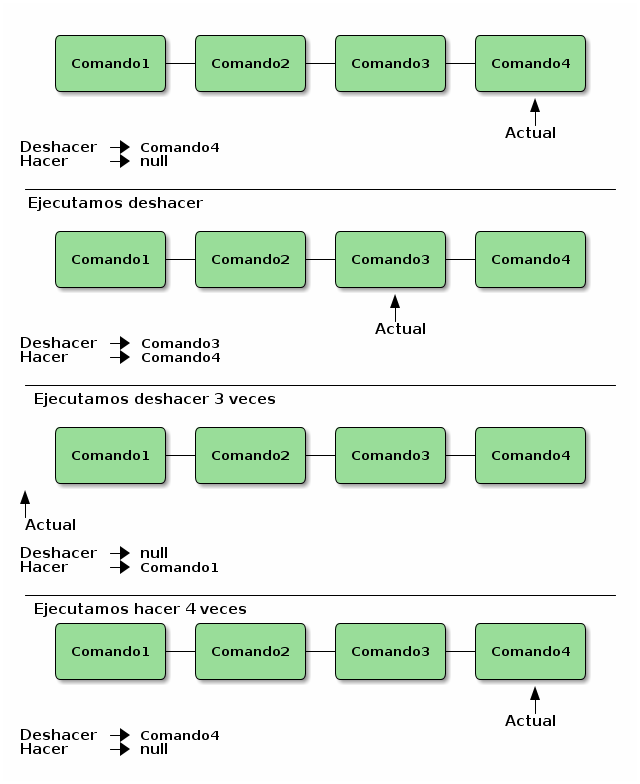
\includegraphics[width=0.7\linewidth]{imagenes/undomangerEjecucion.png}
\caption{Secuencia de ejecución de UndoManager}
\label{fig:undomanager-ejecucion}
\end{figure}

La idea primigenia es posibilitar al usuario final de la aplicación la opción de deshacer y rehacer las acciones ejecutadas en el MindMapJS. UndoManager mantiene en un array los comandos realizados y un puntero (actual) que apunta a la última comando realizado. También disponemos de un limite de comandos(maxComandos) apilados en el historial. 

El interfaz de la clase MM.UndoManager nos permite añadir nuevos comandos al historial, hacer y deshacer, conocer el estado del historial y el nombre del siguiente comando hacer o deshacer. También se le ha incorporado un manejador de eventos para que, los usuarios de la clase puedan saber en todo momento los cambios sufridos en el historial.

\lstinputlisting[language=JavaScript, numbers=left]{../src/undoManager.js}

La clase base de todos los comandos hacer y deshacer es MM.UndoMangaer.ComandoHacerDeshacer. Esta clase implementa un patrón comando con una variante obvia, que en realidad tiene registra dos comandos. Uno para hacer y otro para deshacer. 

\lstinputlisting[language=JavaScript, numbers=left]{../src/undoManager.js}

\section{Concatenación y UglifyJS}
Es conveniente la unificación y compresión de código Javascripts. Con ello, no sólo reducimos el número de peticiones\footnote{Más concretamente peticiones http get}, desde el navegador al servidor, sino que optimizamos los tiempos de carga y respuesta del navegador. Este aspecto es siempre deseable, evitando al usuario final esperas indeseadas.  

Se ha utilizado la herramienta UglifyJS\footnote{En combinación con GruntJS} en MindMapJS, no sólo por tratarse de una librería estándar dentro de herramientas de ofuscación y reducción de código Javascript, sino por los beneficios que nos aporta.

Es sencillo, comprobar que se reduce considerablemente el tiempo, si se concatenan los ficheros Javascript. Por cada fichero Javascript el navegador realiza una petición Get como se puede comprobar en la imagen \ref{fig:carga-desarrollo}.  

\begin{figure}[tbph]
\centering
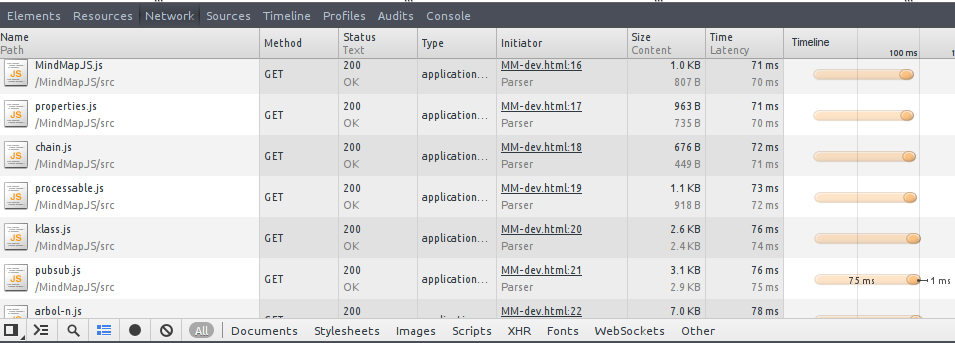
\includegraphics[width=0.9\linewidth]{imagenes/Uglify1.png}
\caption{Carga de ficheros Javascript en desarrollo}
\label{fig:carga-desarrollo}
\end{figure}

Cada solicitud de fichero, por parte del navegador, tiene una latencia de red y un tiempo de carga por parte de navegador que puede provocar, dependiendo de las condiciones y velocidad de la red utilizada, esperas en por parte de usuario final. En la siguiente captura \ref{fig:carga-concatenado}, veremos como al concatenar reducimos el número de peticiones realizadas al servidor y por lo tanto, el tiempo de carga\footnote{Más concretamente a sólo 16ms en un fichero un único fichero de 111Kb.}.

\begin{figure}[tbph]
\centering
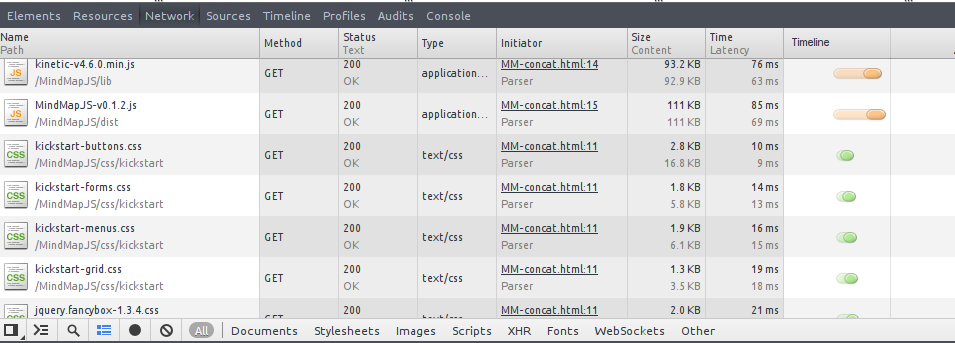
\includegraphics[width=0.9\linewidth]{imagenes/Uglify2.png}
\caption{Carga de ficheros Javascript concatenado}
\label{fig:carga-concatenado}
\end{figure}

Si a su vez comprimimos y reducimos al máximo el tamaño del fichero con UglifyJS, podemos comprobar, en la figura \ref{fig:carga-comprimido}, como el tiempo de carga de la librería se reduce considerablemente. 

\begin{figure}[tbph]
\centering
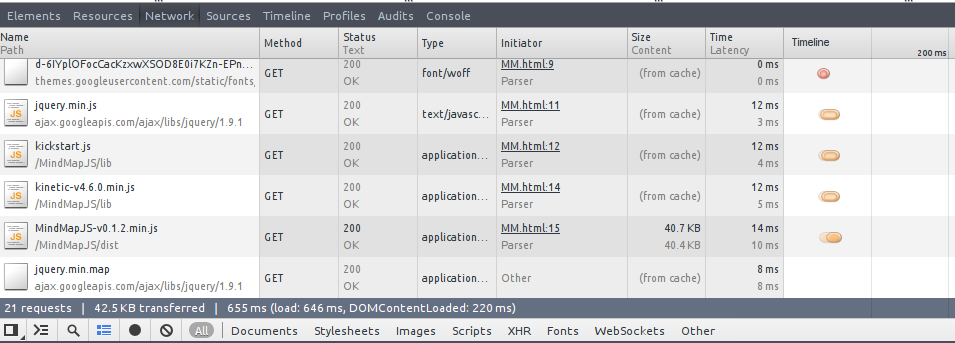
\includegraphics[width=0.9\linewidth]{imagenes/Uglify3.png}
\caption{Carga de ficheros Javascript comprimido}
\label{fig:carga-comprimido}
\end{figure}

Más concretamente, podemos comprobar que el fichero se a reducido desde los 111 Kbytes a 40.7 Kbytes. Es decir, se ha reducido el tamaño del fichero más de 35\% y el tiempo de carga a tan sólo 4 ms. 

Como se puede comprobar es deseable la concatenación y reducción del código en toda aplicación web. Ya que el tiempo de respuesta y la experiencia de usuario mejoran al evitar tiempos muertos en la carga. Sobre todo en sistemas donde el ancho de banda es reducido. 


\section{JsHint}
JsHint es otra herramienta que no debe faltar en ningún desarrollo web. En MindMapJS se ha utilizado continuamente en los periodos de desarrollo. JsHint nos permite comprobar la validez y calidad de nuestro código Javascript, analizando del código fuente y mostrándonos los puntos en los que puede mejorarse desde el punto de vista de las buenas prácticas y código limpio. Evitando pues, errores o posibles errores de interpretación del código fuente.

He utilizado JsHint por que se trata de un estándar utilizado por multitud de desarrollares web y que tiene una gran aceptación por parte de los grandes la programación web. Salvo quizás Douglas Crockford, autor de la herramienta JSLint.

JSLint es un validador de código muy exhaustivo y da muchos falsos positivos. Además tiene muchos detractores, que alegan que los criterios evaluados son bastante subjetivos, sigue los criterios impuestos por Douglas Crockford\footnote{su creador}. Por todo ello, algunos desarrolladores crearon un fork llamado JSHint con el objeto de mejorar las mediciones que eran bastante arbitrarias en JSLint.

\section{KineticJS}
KineticJS es un framework gráfico sobre el canvas de HTML5, permitiendo anidamiento de nodos, capas, filtros, animaciones y manejo de eventos de forma muy sencilla. 

La librería KineticJS tiene en lo alto de la jerarquía de Objetos al escenario que puede tener una o más capas. Cada capa se renderiza en dos canvas, uno para contener los elementos gráficos y otro oculto para agilizar y aclarar la detección de eventos. Cada capa puede contener cualquier elemento gráfico.

\begin{figure}[tbph]
\centering
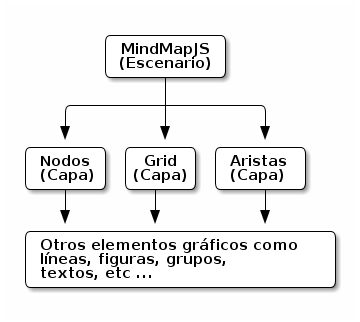
\includegraphics[width=0.6\linewidth]{imagenes/diagrama-kineticjs.png}
\caption{Escenario y modelo de capas KineticJS de MindMapJS}
\label{fig:escenario-capas}
\end{figure}


\subsection{¿Por qué usar KineticJS?}
Entre otras virtudes, lo que más me atrajo a la hora de utilizar KineticJS es:
\begin{itemize}
\item \textbf{Su rendimiento.} Presenta un muy buen rendimiento gráfico. 
\item \textbf{Soporte para capas.} Manejo sencillo de capas permitiendo sobreponer capas.
\item \textbf{API clara y extensible.} Presenta un código claro, orientado a objetos y eventos. Resulta sumamente sencillo extender la librería como se puede ver en el apartado 'Extendiendo KineticJS'.
\item \textbf{Manejo de eventos.} No sólo a nivel de canvas. También a nivel de figura. Soporta multitud de eventos no sólo de escritorio sino también de dispositivos táctiles.
\item \textbf{Continuo desarrollo.} El desarrollo y avance de la librería es notable y tiene una comunidad detrás proporcionando ideas, soluciones, y verificando el desarrollo del la librería.
\end{itemize}

\subsection{Algunos ejemplos sencillos.}
Para todos los ejemplos sobre KineticJS a partir de ahora vamos a utilizar el mismo modelo de página HTML5. En ella, incorporaremos la librería de KineticJS y un contenedor para nuestro lienzo. Una etiqueta div que posteriormente utilizaremos para indicarle a KineticJS donde tiene que pintar.
 
\lstinputlisting[language=HTML, numbers=left]{../test/kineticJS/1_eventos.html}

\subsection{Creando escenarios y capas.}

En este ejemplo vamos a crear un escenario y le incorporaremos una capa donde se dibujará un texto. En la figura \ref{fig:kinetic-ejemplo-escenarios-capas} podemos comprobar el resultado final.

\begin{figure}[tbph]
\centering
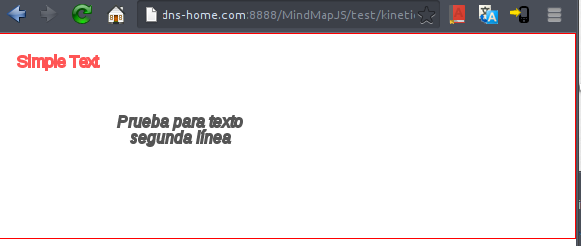
\includegraphics[width=0.6\linewidth]{imagenes/KineticjsEjemplo0.png}
\caption{Ejemplo de Kinetic - uso básico de capas}
\label{fig:kinetic-ejemplo-escenarios-capas}
\end{figure}

\lstinputlisting[language=JavaScript, numbers=left]{../test/kineticJS/0_texto.js}

El ejemplo muestra en la línea 34 como se crea un escenario (Kinetic.Stage) indicando el contenedor dentro nuestro árbol DOM y su dimensiones. A continuación (en la línea 40) creamos una capa (Kintetic.Layer) donde dibujaremos los elementos gráficos que deseamos pintar. Más concretamente se ha creado dos elementos Kinetic.Text y se han incorporado a la capa.

Se trata de un concepto muy utilizado en editores gráficos, por nombrar algunos, como Gimp y PhotoShop. Es exactamente el mismo concepto. En MindMapJS se ha utilizado concretamente tres capas superpuestas en el siguiente orden:
\begin{itemize}
\item \textbf{Capa grid:} muestra la rejilla de fondo.
\item \textbf{Capa aristas:} contiene todas las aristas que interconecta las ideas. 
\item \textbf{Capa nodos:} contiene las ideas que representan el mapa mental.
\end{itemize}


\subsection{Manejo de eventos.}
Como se ha expresado con anterioridad tiene un buen sistema para manejo de eventos tanto de escritorio como touch. En el siguiente ejemplo \ref{fig:kinetic-ejemplo-eventos} podemos ver como manejar eventos sobre objetos con KineticJS.

\begin{figure}[tbph]
\centering
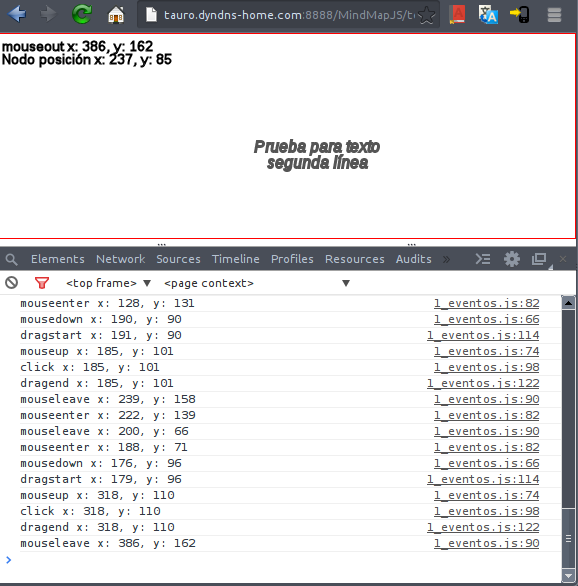
\includegraphics[width=0.6\linewidth]{imagenes/KineticjsEjemplo1.png}
\caption{Ejemplo de Kinetic - eventos}
\label{fig:kinetic-ejemplo-eventos}
\end{figure}

\lstinputlisting[language=JavaScript, numbers=left]{../test/kineticJS/1_eventos.js}

Podemos ver que sigue un modelo de eventos estilo JQuery en el cual nos suscribimos a un evento mediante la fórmula: \footnote{También implementada en MindMapJS} 
\begin{lstlisting}[language=JavaScript, numbers=left]
ElementoGrafico.on('nombreEvento', function () { 
	// Manejo del evento.
});
\end{lstlisting}

Con este modelo, cualquier programador Javascript familiarizado con JQuery entiende como se comporta y sabe de inmediato como utilizarlo.  

Existen otro muchos ejemplos que podemos ver y manipular en la página tutorial de KineticJS\footnote{Tutoriales en http://www.html5canvastutorials.com/kineticjs/html5-canvas-kineticjs-shape-tutorial/}. 

\subsection{Extendiendo KineticJS.}

Existen dos formas de crear y extender KineticJS. La primera es mediante la creación de 'custom shape', se trata de un mecanismo para poder crear figuras que nosotros deseemos pintando directamente en el canvas. La segunda es implementación de una clase y extender su comportamiento dotando a nuestro nuevo elemento gráfico todas la virtudes de cualquier figura KineticJS.

\begin{figure}[tbph]
\centering
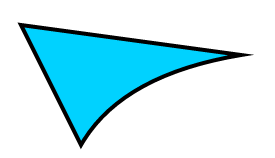
\includegraphics[width=0.6\linewidth]{imagenes/KineticjsEjemplo2.png}
\caption{Ejemplo de Kinetic - custom shape}
\label{fig:kinetic-ejemplo-customshape}
\end{figure}

La creación de 'custom shape' se basa en la implementación de una función (sceneFunc) que será utilizada a la hora de dibujar la figura. Esta función recibe un canvas sobre el que podemos dibujar directamente. 

\begin{lstlisting}[language=JavaScript, numbers=left]
	var stage = new Kinetic.Stage({
        container: 'container',
        width: 578,
        height: 200
    });
    var layer = new Kinetic.Layer();

    var triangle = new Kinetic.Shape({
        sceneFunc: function(context) {
          context.beginPath();
          context.moveTo(200, 50);
          context.lineTo(420, 80);
          context.quadraticCurveTo(300, 100, 260, 170);
          context.closePath();
          context.fillStrokeShape(this);
        },
        fill: '#00D2FF',
        stroke: 'black',
        strokeWidth: 4
    });

    layer.add(triangle);
    stage.add(layer);
\end{lstlisting}

Esta segunda forma de extensión tiene la ventaja de que nos permite crear una clase que podremos reutilizar cada vez que necesitemos. Este mecanismo ha sido el utilizado para crear las aristas de MindMapJS implementando, como podemos comprobar en el siguiente código, una curva beizer para estos propósitos. Se trata, en definitiva, de crear una nueva función constructora y definir su prototipo en el cual no puede faltar la función init y drawFunc. 

\lstinputlisting[language=JavaScript, numbers=left]{../src/beizer.js}

